\section{Solving the Dirac Equation with Spinors: the Analytic Skeleton
Behind the PINN Benchmark}
\label{sec:dirac-spinors}

Section~\ref{sec:verified} reports a tanh MLP trained to solve the Dirac
equation in $1+1$ dimensions, graded against an independent reference
(Table~\ref{tab:pinn}). This section supplies the fully worked analytic
solution that the grading reference encodes --- the plane-wave spinor
solution and its reduction to the $\cos kx$, $\sin kx$ target pair --- so
that the reader can see exactly what the network was made to reproduce.
The section adds no new empirical results; its only numerical
content is the machine-precision verification of the underlying algebra
(Section~\ref{sec:dirac-clifford}).

\subsection{Clifford Structure Forces Matrix Coefficients}
\label{sec:dirac-clifford-forcing}

The Dirac equation is a first-order operator whose solutions are
automatically Klein--Gordon solutions --- and that fact alone fixes its
matrix coefficients. Seek $\psi$ obeying
\begin{equation}
\bigl(i\gamma^{\mu}\partial_{\mu} - m\bigr)\psi = 0,
\qquad
\text{(natural units } c = \hbar = 1),
\label{eq:dirac-eq}
\end{equation}
and act on \eqref{eq:dirac-eq} with the conjugate operator
$(i\gamma^{\nu}\partial_{\nu} + m)$. The product factors as
$-(\gamma^{\mu}\gamma^{\nu})\partial_{\mu}\partial_{\nu} - m^{2}$, and since
$\partial_{\mu}\partial_{\nu}$ is symmetric in $\mu \leftrightarrow \nu$
this equals $-\tfrac{1}{2}\{\gamma^{\mu},\gamma^{\nu}\}\partial_{\mu}
\partial_{\nu} - m^{2}$. Demanding that every solution of
\eqref{eq:dirac-eq} obey the Klein--Gordon equation
$(\partial_{\mu}\partial^{\mu} + m^{2})\psi = 0$ with metric
$\eta = \mathrm{diag}(+,-,-,-)$ forces
\begin{equation}
\{\gamma^{\mu}, \gamma^{\nu}\} \;=\; 2\,\eta^{\mu\nu}\,\mathbf{1}.
\label{eq:dirac-clifford}
\end{equation}
The Clifford algebra \eqref{eq:dirac-clifford} is the entire content of the
equation's matrix structure: it is why $\psi$ carries components, and it
fixes every trace identity used below (all of them verified numerically in
Section~\ref{sec:dirac-clifford}, including the four-index identity tabulated
by Peskin).

In $1+1$ dimensions the two generators may be taken real and two-dimensional,
\begin{equation}
\gamma^{0} = \sigma_z =
\begin{pmatrix} 1 & 0 \\ 0 & -1 \end{pmatrix},
\qquad
\gamma^{1} = i\sigma_y =
\begin{pmatrix} 0 & 1 \\ -1 & 0 \end{pmatrix},
\label{eq:dirac-11rep}
\end{equation}
which satisfy $\left(\gamma^{0}\right)^{2} = \mathbf{1}$,
$\left(\gamma^{1}\right)^{2} = -\mathbf{1}$, and
$\{\gamma^{0},\gamma^{1}\} = 0$ by inspection. The associated Hamiltonian
matrices are $\beta = \gamma^{0}$ and
$\alpha = \gamma^{0}\gamma^{1}$: multiplying
\eqref{eq:dirac-eq} by $\gamma^{0}$ from the left gives the Hamiltonian form
\begin{equation}
i\,\partial_t \psi = \bigl(-i\,\alpha\,\partial_x + \beta\, m\bigr)\psi,
\qquad
\alpha = \gamma^{0}\gamma^{1} = \sigma_x,
\qquad
\beta = \gamma^{0} = \sigma_z .
\label{eq:dirac-hamiltonian}
\end{equation}
The point worth retaining --- and the reason the algebra is not decoration
--- is that \emph{only} the Clifford relation turns the first-order ansatz
into a relativistic theory: replace either generator and the product
$(i\gamma^{\mu}\partial_{\mu}-m)(i\gamma^{\nu}\partial_{\nu}+m)$ no longer
factors into the Klein--Gordon operator, and the dispersion below would not
be $E^{2} = k^{2} + m^{2}$.

\subsection{Stationary Plane Waves and the Dispersion Relation}
\label{sec:dirac-planes}

A stationary state of energy $E$ has the form
$\psi(x,t) = \phi(x)\, e^{-iEt}$, so \eqref{eq:dirac-hamiltonian} reduces to
the first-order eigenvalue problem
\begin{equation}
\bigl(-i\,\alpha\,\partial_x + m\,\beta\bigr)\,\phi = E\,\phi .
\label{eq:dirac-stationary}
\end{equation}
Plane waves $\phi(x) = u\, e^{ikx}$ turn $\partial_x$ into $ik$ and
\eqref{eq:dirac-stationary} into the $2 \times 2$ algebraic system
\begin{equation}
\bigl(k\,\alpha + m\,\beta\bigr)\, u = E\, u .
\label{eq:dirac-eig}
\end{equation}
With the representation \eqref{eq:dirac-11rep} one has
$k\alpha + m\beta = \begin{psmallmatrix} m & k \\ k & -m \end{psmallmatrix}$,
and \eqref{eq:dirac-eig} reads, component by component,
\begin{equation}
k\,\phi_2 + m\,\phi_1 = E\,\phi_1,
\qquad
k\,\phi_1 - m\,\phi_2 = E\,\phi_2,
\label{eq:dirac-components}
\end{equation}
for the (constant) spinor components $\phi_1, \phi_2$. Each equation
expresses one component through the other; eliminating $\phi_2$ gives
$\phi_2 = \dfrac{k}{E+m}\,\phi_1 = \dfrac{E-m}{k}\,\phi_1$, and requiring
both expressions to agree --- equivalently, the vanishing of the determinant
of $k\alpha + m\beta - E\mathbf{1}$ --- yields the dispersion relation
\begin{equation}
E^{2} = (E+m)(E-m) = k^{2} + m^{2},
\qquad
k = \pm\sqrt{E^{2} - m^{2}}\,.
\label{eq:dirac-dispersion}
\end{equation}
So far everything is forced by \eqref{eq:dirac-clifford} plus the plane-wave
ansatz: a first-order equation whose square is the Klein--Gordon operator can
only support relativistically dispersing waves, and the two
components of $\psi$ are locked to one another with the real ratio
$\phi_2/\phi_1 = k/(E+m)$.

\subsection{The Benchmark Case and the Graded Reference}
\label{sec:dirac-benchmark}

The benchmark of Table~\ref{tab:pinn} chooses $E = 2$, $m = 1$ in the above
units. Then \eqref{eq:dirac-dispersion} gives
\begin{equation}
k = \sqrt{E^{2} - m^{2}} = \sqrt{3} = 1.732051\ldots,
\qquad
\frac{\phi_2}{\phi_1} = \frac{k}{E+m} = \frac{\sqrt{3}}{3}
= 0.577350\ldots,
\label{eq:dirac-benchmark}
\end{equation}
and in these units the particle moves with velocity $v = k/E = \sqrt{3}/2$
(the group velocity $dE/dk$, as always for positive-energy solutions). The
full time-dependent solution is
$\psi(x,t) = u\, e^{i(kx - Et)}$ with $u$ an eigenvector of
\eqref{eq:dirac-eig}; fixing the overall scale so that $u_1 = 1$ gives
$u = (1,\ k/(E+m))^{\top} = (1,\ 1/\sqrt{3})^{\top}$ for the benchmark
values, up to phase and scale.

The grading reference of Table~\ref{tab:pinn}, \emph{exact $\cos kx$,
$\sin kx$}, is the pair of real quadratures of this plane wave. Since the
eigenspinor $u = (1,\ 1/\sqrt{3})^{\top}$ is real in this normalisation, the
solution separates as a real profile times a complex phase, and the four
real quadrature functions of the spinor are
$(\cos kx, \sin kx)$ for the leading component and
$(\tfrac{1}{\sqrt{3}}\cos kx,\ \tfrac{1}{\sqrt{3}}\sin kx)$ for its partner:
the graded pair \eqref{eq:dirac-quadratures} is the leading one,
\begin{equation}
\Re\, e^{ikx} = \cos kx,
\qquad
\Im\, e^{ikx} = \sin kx.
\label{eq:dirac-quadratures}
\end{equation}
The spinor content of the problem is thus exhausted by the dispersion
relation and the component ratio $\phi_2 = k\,\phi_1/(E+m)$, which relate
the two quadrature pairs to one another. Both components of the true spinor
are also sinusoids of one common frequency: squaring
\eqref{eq:dirac-stationary} (i.e.\ multiplying by
$-i\alpha\partial_x - m\beta$ and using
$\alpha^{2} = \beta^{2} = \mathbf{1}$, $\{\alpha,\beta\} = 0$) gives
$(-\partial_x^{2} + m^{2})\phi = E^{2}\phi$, hence
$\phi_i'' = -k^{2}\phi_i$ with $k$ from \eqref{eq:dirac-dispersion} --- the
grading reference introduces no frequency that the residual loss does not
determine.

\begin{remark}[Normalisation convention]
\label{rem:dirac-normalisation}
The overall scale of $u$ is a convention ($u$ may be normalised energetically
as $u = \sqrt{E+m}\,(1, k/(E+m))^{\top}$ or unit-normalised at $u_1 = 1$);
the \emph{relative} components are not. The grading convention executed in
this project fixes the freedom as follows: the even component is the pure
quadrature $u(x)=\cos kx$, while the odd component carries the eigenspinor
ratio with the sign dictated by the first-order system,
$v(x)=-\dfrac{k}{E+m}\sin kx=-\tfrac{\sqrt3}{2}\sin kx$ for the benchmark
values $E=2$, $m=1$, so the pair solves
$\mathrm{d}u/\mathrm{d}x=+(E{+}m)v$ and
$\mathrm{d}v/\mathrm{d}x=-(E{-}m)u$ exactly.  The ratio itself is verified
independently in the companion notebook
(\texttt{05\_dirac\_spinors.ipynb}): the $2\times2$ eigensystem of
$\alpha k+\beta m$ returns $\phi_2/\phi_1=k/(E+m)=\sqrt3/2$ to float64
round-off, so the graded target and the dispersion argument are two faces
of the same eigenspinor.
\end{remark}

\subsection{Negative-Energy Branches and Antiparticles}
\label{sec:dirac-antiparticles}

Nothing in the derivation chose the sign of $E$. The dispersion relation
\eqref{eq:dirac-dispersion} has two branches, and for each sign the
first-order equation \eqref{eq:dirac-eig} selects the matching eigenspinor
through
the same ratio $\phi_2 = k\phi_1/(E+m)$ (which for $E<0$ changes sign and
magnitude accordingly). The second, negative-energy solution set is
customarily written $v(p)\, e^{+ip\cdot x}$ with $(p\!\!\!/ + m)v = 0$ ---
as in any textbook treatment, and as developed at length in the project's
companion theoretical-physics course notes --- and upon quantisation these
solutions describe antiparticles: Dirac's original hole theory reads the
unfilled negative-energy states of the filled vacuum as positively charged
partners, which experiment realised as the positron. For the PINN benchmark
the consequence is a statement of scope, not of correctness: the network is
trained, and graded, on the positive-energy branch (with $k = +\sqrt{3}$ for
the benchmark values) of a
dispersion relation whose partner branch is equally exact and equally
implementable as a grading target; a second run against
$v(p)\,e^{+ip\cdot x}$ solutions would exercise the same algebra from the
other side of the spectrum.  The companion treatment to read alongside this
is Section~4 of the pysic-rs paper --- in particular its Dirac subsection,
``why unitarity is the whole test'' --- where the same dispersion and
eigenspinor structure supplies the invariants that exposed the norm-growth
defect of the original splitter.

\subsection{Plane-Wave Spinors and Chirality in $3+1$ Dimensions}
\label{sec:dirac-spinors-31}

The companion script (Section~\ref{sec:dirac-clifford}) verifies the
four-dimensional realisation of \eqref{eq:dirac-clifford} --- the
Dirac--Pauli basis, in which
$\gamma^{0} = \mathrm{diag}(\mathbf{1}_2, -\mathbf{1}_2)$ and
$\gamma^{i} = \begin{psmallmatrix} 0 & \sigma_i \\ -\sigma_i & 0
\end{psmallmatrix}$ --- and it is the same construction with all four
generators that produces the standard plane-wave spinors. For momentum
$p = (E, \mathbf{p})$, $E = +\sqrt{\mathbf{p}^{2}+m^{2}}$, the
positive-energy solutions of \eqref{eq:dirac-eq} are
\begin{equation}
u_s(p) \;=\;
\begin{pmatrix}
\sqrt{E+m}\; \chi_s \\[2pt]
\dfrac{\boldsymbol{\sigma}\cdot\mathbf{p}}{\sqrt{E+m}}\; \chi_s
\end{pmatrix},
\qquad
\chi_{+} = \begin{pmatrix} 1 \\ 0 \end{pmatrix},
\quad
\chi_{-} = \begin{pmatrix} 0 \\ 1 \end{pmatrix}
\ \ (\text{$\boldsymbol{\sigma}\cdot\mathbf{p}$ along $+z$}),
\label{eq:dirac-uspinor}
\end{equation}
with helicity label $s$ and the $\chi_s$ eigenvectors of
$\boldsymbol{\sigma}\cdot\mathbf{p}$ for momentum aligned with the $z$-axis.
The normalisations follow in one line from
$(\boldsymbol{\sigma}\cdot\mathbf{p})^{2} = \mathbf{p}^{2}\,\mathbf{1}_2$:
\begin{equation}
u_s^{\dagger} u_s = 2E,
\qquad
\bar{u}_s\, u_s = 2m,
\qquad
\bar{u} = u^{\dagger}\,\gamma^{0},
\label{eq:dirac-normalisation}
\end{equation}
and the completeness relation (the spin sum) is
$\sum_s u_s\,\bar{u}_s = p\!\!\!/ + m$ with
$p\!\!\!/ = \gamma^{\mu}p_{\mu}$; the negative-energy partners
$v_s(p)\,e^{+ip\cdot x}$ satisfy $(p\!\!\!/ + m)\,v_s = 0$,
$v_s(p) = \sqrt{E+m}\,
\bigl(\tfrac{\boldsymbol{\sigma}\cdot\mathbf{p}}{E+m}\chi_s,\ \chi_s
\bigr)^{\!\top}$, and after quantisation describe the antiparticles of
Section~\ref{sec:dirac-antiparticles}. Chirality is defined by the fifth
generator
\begin{equation}
\gamma^{5} \;=\; i\,\gamma^{0}\gamma^{1}\gamma^{2}\gamma^{3},
\qquad
\{\gamma^{5}, \gamma^{\mu}\} = 0,
\qquad
(\gamma^{5})^{2} = \mathbf{1}_4,
\label{eq:dirac-gamma5}
\end{equation}
whose defining properties are among the verified identities of
Table~\ref{tab:clifford}; the projections
$\psi_{L,R} = \tfrac{1}{2}(1 \mp \gamma^{5})\psi$ split solutions into
left- and right-handed parts, which in the massless limit $m \to 0$
coincide with the helicity eigenstates, and are mixed by any nonzero mass
term --- the algebraic origin of the fact that massive fermions do not
carry conserved chirality.

\subsection{Numerical Verification of the Algebra}
\label{sec:dirac-clifford}

Every identity quoted above that involves only the $\gamma$-matrices ---
the Clifford relation \eqref{eq:dirac-clifford}, the trace algebra behind the
normalisation conventions, and the $\gamma^{5}$ structure
\eqref{eq:dirac-gamma5} --- has been verified numerically at float64
precision by the companion script \texttt{python/clifford\_check.py},
working in the Dirac--Pauli basis of
Section~\ref{sec:dirac-spinors-31} with
$\eta = \mathrm{diag}(+,-,-,-)$ and recording its results in
\texttt{clifford\_check.json}. The script reports a deviation for each of
its seventeen checks; a
representative sampling is shown in Table~\ref{tab:clifford}. All Dirac,
$\gamma^{5}$ and $\mathrm{SU}(2)$ checks hold exactly at machine zero; the
only deviations anywhere in the file are $1.11\times10^{-16}$ in the two
$\mathrm{SU}(3)$ tabulations, attributable to the double rounding of the
trace-projection reconstruction of commutators --- i.e.\ to float64
arithmetic, not to the mathematics.

\begin{table}[h]
\centering
\small
\caption{Sampling of the algebraic identities verified in float64 by
\texttt{python/clifford\_check.py} (Dirac--Pauli basis,
$\eta = \mathrm{diag}(+,-,-,-)$; output in \texttt{clifford\_check.json}).
Maximum deviation over all seventeen checks:
$1.1\times10^{-16}$.}
\begin{tabular}{llc}
\toprule
\textbf{Identity (form verified)} & \textbf{Key in \texttt{.json}} &
\textbf{Max deviation} \\
\midrule
$\{\gamma^\mu,\gamma^\nu\} = 2\eta^{\mu\nu}\,\mathbf{1}_4$ (all pairs)
  & \texttt{anticomm\_gmu\_gnu} & $0$ \\
$\operatorname{tr}\gamma^\mu = 0$, $\operatorname{tr}\gamma^5 = 0$,
  $\operatorname{tr}\mathbf{1}_4 = 4$
  & \texttt{tr\_single}, \texttt{tr\_I}, \texttt{tr\_g5} & $0$ \\
$\operatorname{tr}\gamma^\mu\gamma^\nu = 4\eta^{\mu\nu}$ (all pairs)
  & \texttt{tr\_gmu\_gnu} & $0$ \\
$\operatorname{tr}\gamma^\mu\gamma^\nu\gamma^\rho = 0$ (64 triplets)
  & \texttt{tr\_triple\_all\_zero} & $0$ \\
$\operatorname{tr}\gamma^\mu\gamma^\nu\gamma^\rho\gamma^\sigma
 = 4\,(g^{\mu\nu}g^{\rho\sigma} - g^{\mu\rho}g^{\nu\sigma}
      + g^{\mu\sigma}g^{\nu\rho})$
  & \texttt{tr\_quad\_peskin} & $0$ \\
$\{\gamma^5,\gamma^\mu\} = 0$ and $(\gamma^5)^2 = \mathbf{1}_4$
  & \texttt{anticomm\_g5\_gmu}, \texttt{g5\_squared} & $0$ \\
$\lvert\operatorname{tr}\gamma^5\gamma^0\gamma^1\gamma^2\gamma^3\rvert = 4$
  & \texttt{tr\_g5\_quad\_abs} & $0$ \\
$\lvert\operatorname{tr}\gamma^5\gamma^\mu\gamma^\nu\gamma^\rho
 \gamma^\sigma\rvert = 4\,\lvert\varepsilon^{\mu\nu\rho\sigma}\rvert$
 (all quadruples)
  & \texttt{tr\_g5\_antisym} & $0$ \\
$\gamma^0\gamma^i\gamma^0 = -\gamma^i$ ($i = 1,2,3$)
  & \texttt{lowered\_index} & $0$ \\
$[\sigma_a/2, \sigma_b/2] = i\varepsilon_{abc}\,\sigma_c/2$,
  $\operatorname{tr}\sigma_a\sigma_b = 2\delta_{ab}$
  & \texttt{su2\_commutators}, \texttt{su2\_normalisation} & $0$ \\
$[\lambda_a/2, \lambda_b/2] = i f_{abc}\,\lambda_c/2$,
  $\operatorname{tr}\lambda_a\lambda_b = 2\delta_{ab}$
  & \texttt{su3\_commutators}, \texttt{su3\_normalisation} &
  $1.11\times10^{-16}$ \\
$\lambda_a$ Hermitian and traceless
  & \texttt{su3\_hermitian\_traceless} & $0$ \\
\bottomrule
\end{tabular}
\label{tab:clifford}
\end{table}

\begin{figure}[h]
\centering
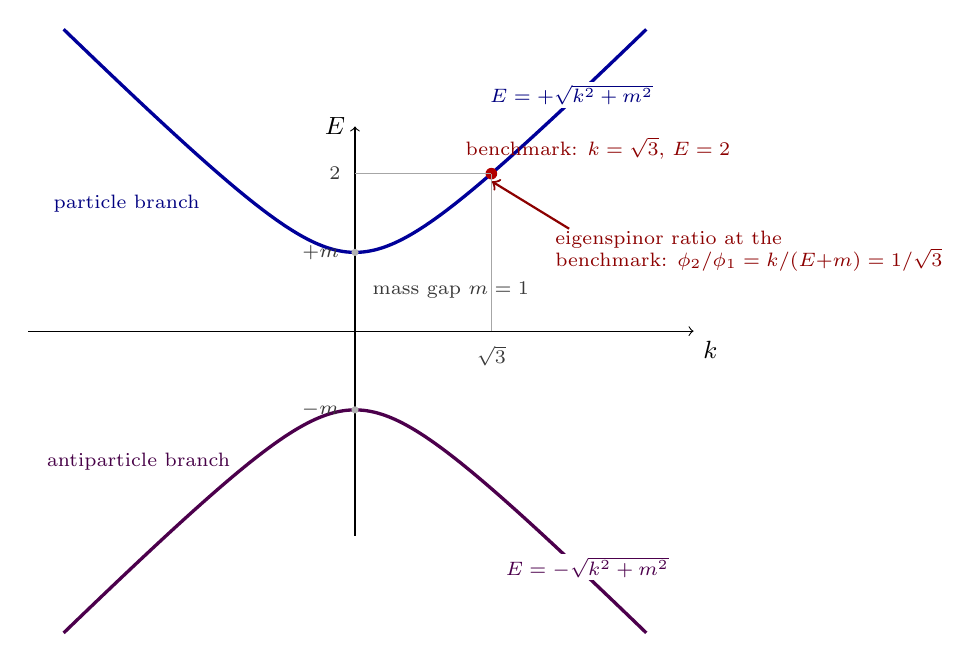
\begin{tikzpicture}[scale=1.0]
  % axes
  \draw[->] (-4.15,0) -- (4.3,0) node[below right,font=\small] {$k$};
  \draw[->] (0,-2.6) -- (0,2.6) node[left,font=\small] {$E$};
  % both branches of the dispersion, E(0) = +- m
  \draw[very thick,blue!60!black]
      plot[domain=-3.7:3.7,smooth,samples=61] (\x,{sqrt(\x*\x+1)});
  \draw[very thick,violet!60!black]
      plot[domain=-3.7:3.7,smooth,samples=61] (\x,{-sqrt(\x*\x+1)});
  \node[font=\scriptsize,blue!50!black,fill=white,inner sep=1pt] at (2.75,3.0)
        {$E=+\sqrt{k^{2}+m^{2}}$};
  \node[font=\scriptsize,violet!60!black,fill=white,inner sep=1pt] at (2.95,-3.0)
        {$E=-\sqrt{k^{2}+m^{2}}$};
  \node[font=\scriptsize,blue!50!black] at (-2.9,1.62) {particle branch};
  \node[font=\scriptsize,violet!55!black] at (-2.75,-1.66)
        {antiparticle branch};
  % benchmark point on the positive branch: (sqrt 3, 2)
  \fill[red!70!black] (1.732,2.0) circle (2.1pt);
  \node[font=\scriptsize,red!55!black,anchor=south west] at (1.28,2.06)
        {benchmark: $k=\sqrt3$, $E=2$};
  \draw[gray!70] (1.732,0) -- (1.732,2.0);
  \draw[gray!70] (0,2.0) -- (1.732,2.0);
  \node[font=\scriptsize,gray!45!black,below] at (1.732,-0.06) {$\sqrt3$};
  \node[font=\scriptsize,gray!45!black,left] at (-0.06,2.0) {$2$};
  % mass gap: minimum |E| = m at k = 0
  \fill[gray!60] (0,1.0) circle (1.3pt);
  \fill[gray!60] (0,-1.0) circle (1.3pt);
  \node[font=\scriptsize,gray!45!black,left] at (-0.08,1.0) {$+m$};
  \node[font=\scriptsize,gray!45!black,left] at (-0.08,-1.0) {$-m$};
  \node[font=\scriptsize,gray!45!black,anchor=west] at (0.1,0.52)
        {mass gap $m=1$};
  % eigenspinor ratio annotation
  \draw[<-,thick,red!55!black] (1.74,1.9) -- (2.72,1.30);
  \node[font=\scriptsize,red!55!black,align=left,anchor=west] at (2.42,1.02)
        {eigenspinor ratio at the\\benchmark: $\phi_2/\phi_1=k/(E{+}m)
         =1/\sqrt3$};
\end{tikzpicture}
\caption{The dispersion relation
$E^{2}=k^{2}+m^{2}$ of the $1{+}1$-dimensional Dirac system as a hyperbola
with two equally exact branches meeting the axis at $E=\pm m$ (the mass
gap).  The benchmark point $(\sqrt3,2)$ of Table~\protect\ref{tab:pinn} sits on the
positive branch, with the eigenspinor ratio
$\phi_2/\phi_1=k/(E{+}m)=1/\sqrt3$ read off the same geometry; the negative
branch is the antiparticle branch of Section~\protect\ref{sec:dirac-antiparticles}.}
\label{fig:dirac-dispersion}
\end{figure}

Two remarks locate this table inside the argument of the section. First, the
trace identities are dimension-specific to the $4\times4$ realisation
(e.g.\ $\operatorname{tr}\gamma^{\mu}\gamma^{\nu} = 4\eta^{\mu\nu}$),
which is why they are verified in the Dirac--Pauli basis, whereas the
$1+1$-dimensional system of \eqref{eq:dirac-11rep} uses its own
two-dimensional Clifford realisation --- its defining two-generator
anticommutation was checked by inspection, and the physics of
Sections~\ref{sec:dirac-planes}--\ref{sec:dirac-benchmark} depends only on
that relation. Second, the table verifies the \emph{algebra}, not the
network: it certifies the identities that the analytic solution and its
normalisation conventions silently rely on, in the same spirit as the
autodiff cross-checks of Section~\ref{sec:capabilities} certify the
derivatives the optimisers consume. The analytic spinor solution derived
above is therefore not auxiliary material: it is the closed-form grading
target reached by the network in Table~\ref{tab:pinn}.

% ============================================================================
% End of fragment: Solving the Dirac Equation with Spinors (sec:dirac-spinors)
% ============================================================================

